% Options for packages loaded elsewhere
% Options for packages loaded elsewhere
\PassOptionsToPackage{unicode}{hyperref}
\PassOptionsToPackage{hyphens}{url}
\PassOptionsToPackage{dvipsnames,svgnames,x11names}{xcolor}
%
\documentclass[
  letterpaper,
  DIV=11,
  numbers=noendperiod]{scrartcl}
\usepackage{xcolor}
\usepackage{amsmath,amssymb}
\setcounter{secnumdepth}{-\maxdimen} % remove section numbering
\usepackage{iftex}
\ifPDFTeX
  \usepackage[T1]{fontenc}
  \usepackage[utf8]{inputenc}
  \usepackage{textcomp} % provide euro and other symbols
\else % if luatex or xetex
  \usepackage{unicode-math} % this also loads fontspec
  \defaultfontfeatures{Scale=MatchLowercase}
  \defaultfontfeatures[\rmfamily]{Ligatures=TeX,Scale=1}
\fi
\usepackage{lmodern}
\ifPDFTeX\else
  % xetex/luatex font selection
\fi
% Use upquote if available, for straight quotes in verbatim environments
\IfFileExists{upquote.sty}{\usepackage{upquote}}{}
\IfFileExists{microtype.sty}{% use microtype if available
  \usepackage[]{microtype}
  \UseMicrotypeSet[protrusion]{basicmath} % disable protrusion for tt fonts
}{}
\makeatletter
\@ifundefined{KOMAClassName}{% if non-KOMA class
  \IfFileExists{parskip.sty}{%
    \usepackage{parskip}
  }{% else
    \setlength{\parindent}{0pt}
    \setlength{\parskip}{6pt plus 2pt minus 1pt}}
}{% if KOMA class
  \KOMAoptions{parskip=half}}
\makeatother
% Make \paragraph and \subparagraph free-standing
\makeatletter
\ifx\paragraph\undefined\else
  \let\oldparagraph\paragraph
  \renewcommand{\paragraph}{
    \@ifstar
      \xxxParagraphStar
      \xxxParagraphNoStar
  }
  \newcommand{\xxxParagraphStar}[1]{\oldparagraph*{#1}\mbox{}}
  \newcommand{\xxxParagraphNoStar}[1]{\oldparagraph{#1}\mbox{}}
\fi
\ifx\subparagraph\undefined\else
  \let\oldsubparagraph\subparagraph
  \renewcommand{\subparagraph}{
    \@ifstar
      \xxxSubParagraphStar
      \xxxSubParagraphNoStar
  }
  \newcommand{\xxxSubParagraphStar}[1]{\oldsubparagraph*{#1}\mbox{}}
  \newcommand{\xxxSubParagraphNoStar}[1]{\oldsubparagraph{#1}\mbox{}}
\fi
\makeatother

\usepackage{color}
\usepackage{fancyvrb}
\newcommand{\VerbBar}{|}
\newcommand{\VERB}{\Verb[commandchars=\\\{\}]}
\DefineVerbatimEnvironment{Highlighting}{Verbatim}{commandchars=\\\{\}}
% Add ',fontsize=\small' for more characters per line
\usepackage{framed}
\definecolor{shadecolor}{RGB}{241,243,245}
\newenvironment{Shaded}{\begin{snugshade}}{\end{snugshade}}
\newcommand{\AlertTok}[1]{\textcolor[rgb]{0.68,0.00,0.00}{#1}}
\newcommand{\AnnotationTok}[1]{\textcolor[rgb]{0.37,0.37,0.37}{#1}}
\newcommand{\AttributeTok}[1]{\textcolor[rgb]{0.40,0.45,0.13}{#1}}
\newcommand{\BaseNTok}[1]{\textcolor[rgb]{0.68,0.00,0.00}{#1}}
\newcommand{\BuiltInTok}[1]{\textcolor[rgb]{0.00,0.23,0.31}{#1}}
\newcommand{\CharTok}[1]{\textcolor[rgb]{0.13,0.47,0.30}{#1}}
\newcommand{\CommentTok}[1]{\textcolor[rgb]{0.37,0.37,0.37}{#1}}
\newcommand{\CommentVarTok}[1]{\textcolor[rgb]{0.37,0.37,0.37}{\textit{#1}}}
\newcommand{\ConstantTok}[1]{\textcolor[rgb]{0.56,0.35,0.01}{#1}}
\newcommand{\ControlFlowTok}[1]{\textcolor[rgb]{0.00,0.23,0.31}{\textbf{#1}}}
\newcommand{\DataTypeTok}[1]{\textcolor[rgb]{0.68,0.00,0.00}{#1}}
\newcommand{\DecValTok}[1]{\textcolor[rgb]{0.68,0.00,0.00}{#1}}
\newcommand{\DocumentationTok}[1]{\textcolor[rgb]{0.37,0.37,0.37}{\textit{#1}}}
\newcommand{\ErrorTok}[1]{\textcolor[rgb]{0.68,0.00,0.00}{#1}}
\newcommand{\ExtensionTok}[1]{\textcolor[rgb]{0.00,0.23,0.31}{#1}}
\newcommand{\FloatTok}[1]{\textcolor[rgb]{0.68,0.00,0.00}{#1}}
\newcommand{\FunctionTok}[1]{\textcolor[rgb]{0.28,0.35,0.67}{#1}}
\newcommand{\ImportTok}[1]{\textcolor[rgb]{0.00,0.46,0.62}{#1}}
\newcommand{\InformationTok}[1]{\textcolor[rgb]{0.37,0.37,0.37}{#1}}
\newcommand{\KeywordTok}[1]{\textcolor[rgb]{0.00,0.23,0.31}{\textbf{#1}}}
\newcommand{\NormalTok}[1]{\textcolor[rgb]{0.00,0.23,0.31}{#1}}
\newcommand{\OperatorTok}[1]{\textcolor[rgb]{0.37,0.37,0.37}{#1}}
\newcommand{\OtherTok}[1]{\textcolor[rgb]{0.00,0.23,0.31}{#1}}
\newcommand{\PreprocessorTok}[1]{\textcolor[rgb]{0.68,0.00,0.00}{#1}}
\newcommand{\RegionMarkerTok}[1]{\textcolor[rgb]{0.00,0.23,0.31}{#1}}
\newcommand{\SpecialCharTok}[1]{\textcolor[rgb]{0.37,0.37,0.37}{#1}}
\newcommand{\SpecialStringTok}[1]{\textcolor[rgb]{0.13,0.47,0.30}{#1}}
\newcommand{\StringTok}[1]{\textcolor[rgb]{0.13,0.47,0.30}{#1}}
\newcommand{\VariableTok}[1]{\textcolor[rgb]{0.07,0.07,0.07}{#1}}
\newcommand{\VerbatimStringTok}[1]{\textcolor[rgb]{0.13,0.47,0.30}{#1}}
\newcommand{\WarningTok}[1]{\textcolor[rgb]{0.37,0.37,0.37}{\textit{#1}}}

\usepackage{longtable,booktabs,array}
\newcounter{none} % for unnumbered tables
\usepackage{calc} % for calculating minipage widths
% Correct order of tables after \paragraph or \subparagraph
\usepackage{etoolbox}
\makeatletter
\patchcmd\longtable{\par}{\if@noskipsec\mbox{}\fi\par}{}{}
\makeatother
% Allow footnotes in longtable head/foot
\IfFileExists{footnotehyper.sty}{\usepackage{footnotehyper}}{\usepackage{footnote}}
\makesavenoteenv{longtable}
\usepackage{graphicx}
\makeatletter
\newsavebox\pandoc@box
\newcommand*\pandocbounded[1]{% scales image to fit in text height/width
  \sbox\pandoc@box{#1}%
  \Gscale@div\@tempa{\textheight}{\dimexpr\ht\pandoc@box+\dp\pandoc@box\relax}%
  \Gscale@div\@tempb{\linewidth}{\wd\pandoc@box}%
  \ifdim\@tempb\p@<\@tempa\p@\let\@tempa\@tempb\fi% select the smaller of both
  \ifdim\@tempa\p@<\p@\scalebox{\@tempa}{\usebox\pandoc@box}%
  \else\usebox{\pandoc@box}%
  \fi%
}
% Set default figure placement to htbp
\def\fps@figure{htbp}
\makeatother





\setlength{\emergencystretch}{3em} % prevent overfull lines

\providecommand{\tightlist}{%
  \setlength{\itemsep}{0pt}\setlength{\parskip}{0pt}}



 


\KOMAoption{captions}{tableheading}
\makeatletter
\@ifpackageloaded{caption}{}{\usepackage{caption}}
\AtBeginDocument{%
\ifdefined\contentsname
  \renewcommand*\contentsname{Table of contents}
\else
  \newcommand\contentsname{Table of contents}
\fi
\ifdefined\listfigurename
  \renewcommand*\listfigurename{List of Figures}
\else
  \newcommand\listfigurename{List of Figures}
\fi
\ifdefined\listtablename
  \renewcommand*\listtablename{List of Tables}
\else
  \newcommand\listtablename{List of Tables}
\fi
\ifdefined\figurename
  \renewcommand*\figurename{Figure}
\else
  \newcommand\figurename{Figure}
\fi
\ifdefined\tablename
  \renewcommand*\tablename{Table}
\else
  \newcommand\tablename{Table}
\fi
}
\@ifpackageloaded{float}{}{\usepackage{float}}
\floatstyle{ruled}
\@ifundefined{c@chapter}{\newfloat{codelisting}{h}{lop}}{\newfloat{codelisting}{h}{lop}[chapter]}
\floatname{codelisting}{Listing}
\newcommand*\listoflistings{\listof{codelisting}{List of Listings}}
\makeatother
\makeatletter
\makeatother
\makeatletter
\@ifpackageloaded{caption}{}{\usepackage{caption}}
\@ifpackageloaded{subcaption}{}{\usepackage{subcaption}}
\makeatother
\usepackage{bookmark}
\IfFileExists{xurl.sty}{\usepackage{xurl}}{} % add URL line breaks if available
\urlstyle{same}
\hypersetup{
  pdftitle={ETC5513: Collaborative and Reproducible Practices},
  pdfauthor={Tushar Dhanorkar},
  colorlinks=true,
  linkcolor={blue},
  filecolor={Maroon},
  citecolor={Blue},
  urlcolor={Blue},
  pdfcreator={LaTeX via pandoc}}


\title{ETC5513: Collaborative and Reproducible Practices}
\author{Tushar Dhanorkar}
\date{}
\begin{document}
\maketitle


\subsection{Assignment 2}\label{assignment-2}

This guide walk through ten practical steps demonstrating the use of
Git, Github and Command line interface for Version control and
collaboration. Each step explains what to do and why does this matters.

\paragraph{\texorpdfstring{\textbf{Step 1: Create the RStudio
Project}}{Step 1: Create the RStudio Project}}\label{step-1-create-the-rstudio-project}

\paragraph{What is an RStudio
Project?}\label{what-is-an-rstudio-project}

An RStudio Project is simply a \textbf{folder on your computer} that
RStudio treats as a self-contained workspace. It keeps all your files,
settings, and working directory in one place. When you open the project,
RStudio automatically sets the working directory to that folder ---
which is important for reproducibility.

Part A: Create the RStudio Project

\begin{enumerate}
\def\labelenumi{\arabic{enumi}.}
\item
  Open \textbf{RStudio}
\item
  Click \textbf{File} in the top menu → \textbf{New Project.}
\item
  A dialog box appears. Choose \textbf{New Directory}
\item
  Then choose \textbf{New Project}
\item
  You'll see a form:

  \begin{itemize}
  \item
    \textbf{Directory name:} type 02\_etc5513
  \item
    \textbf{Create project as subdirectory of:} choose a location on
    your computer (e.g.~your Desktop or Documents folder)
  \end{itemize}
\item
  Click \textbf{Create Project}
\item
  RStudio will reload and you'll now be inside your new project. You'll
  notice the top-right corner of RStudio shows your project name. In the
  Files panel (bottom-right), you'll see one file:
  \texttt{assignment2.Rproj}
\end{enumerate}

\pandocbounded{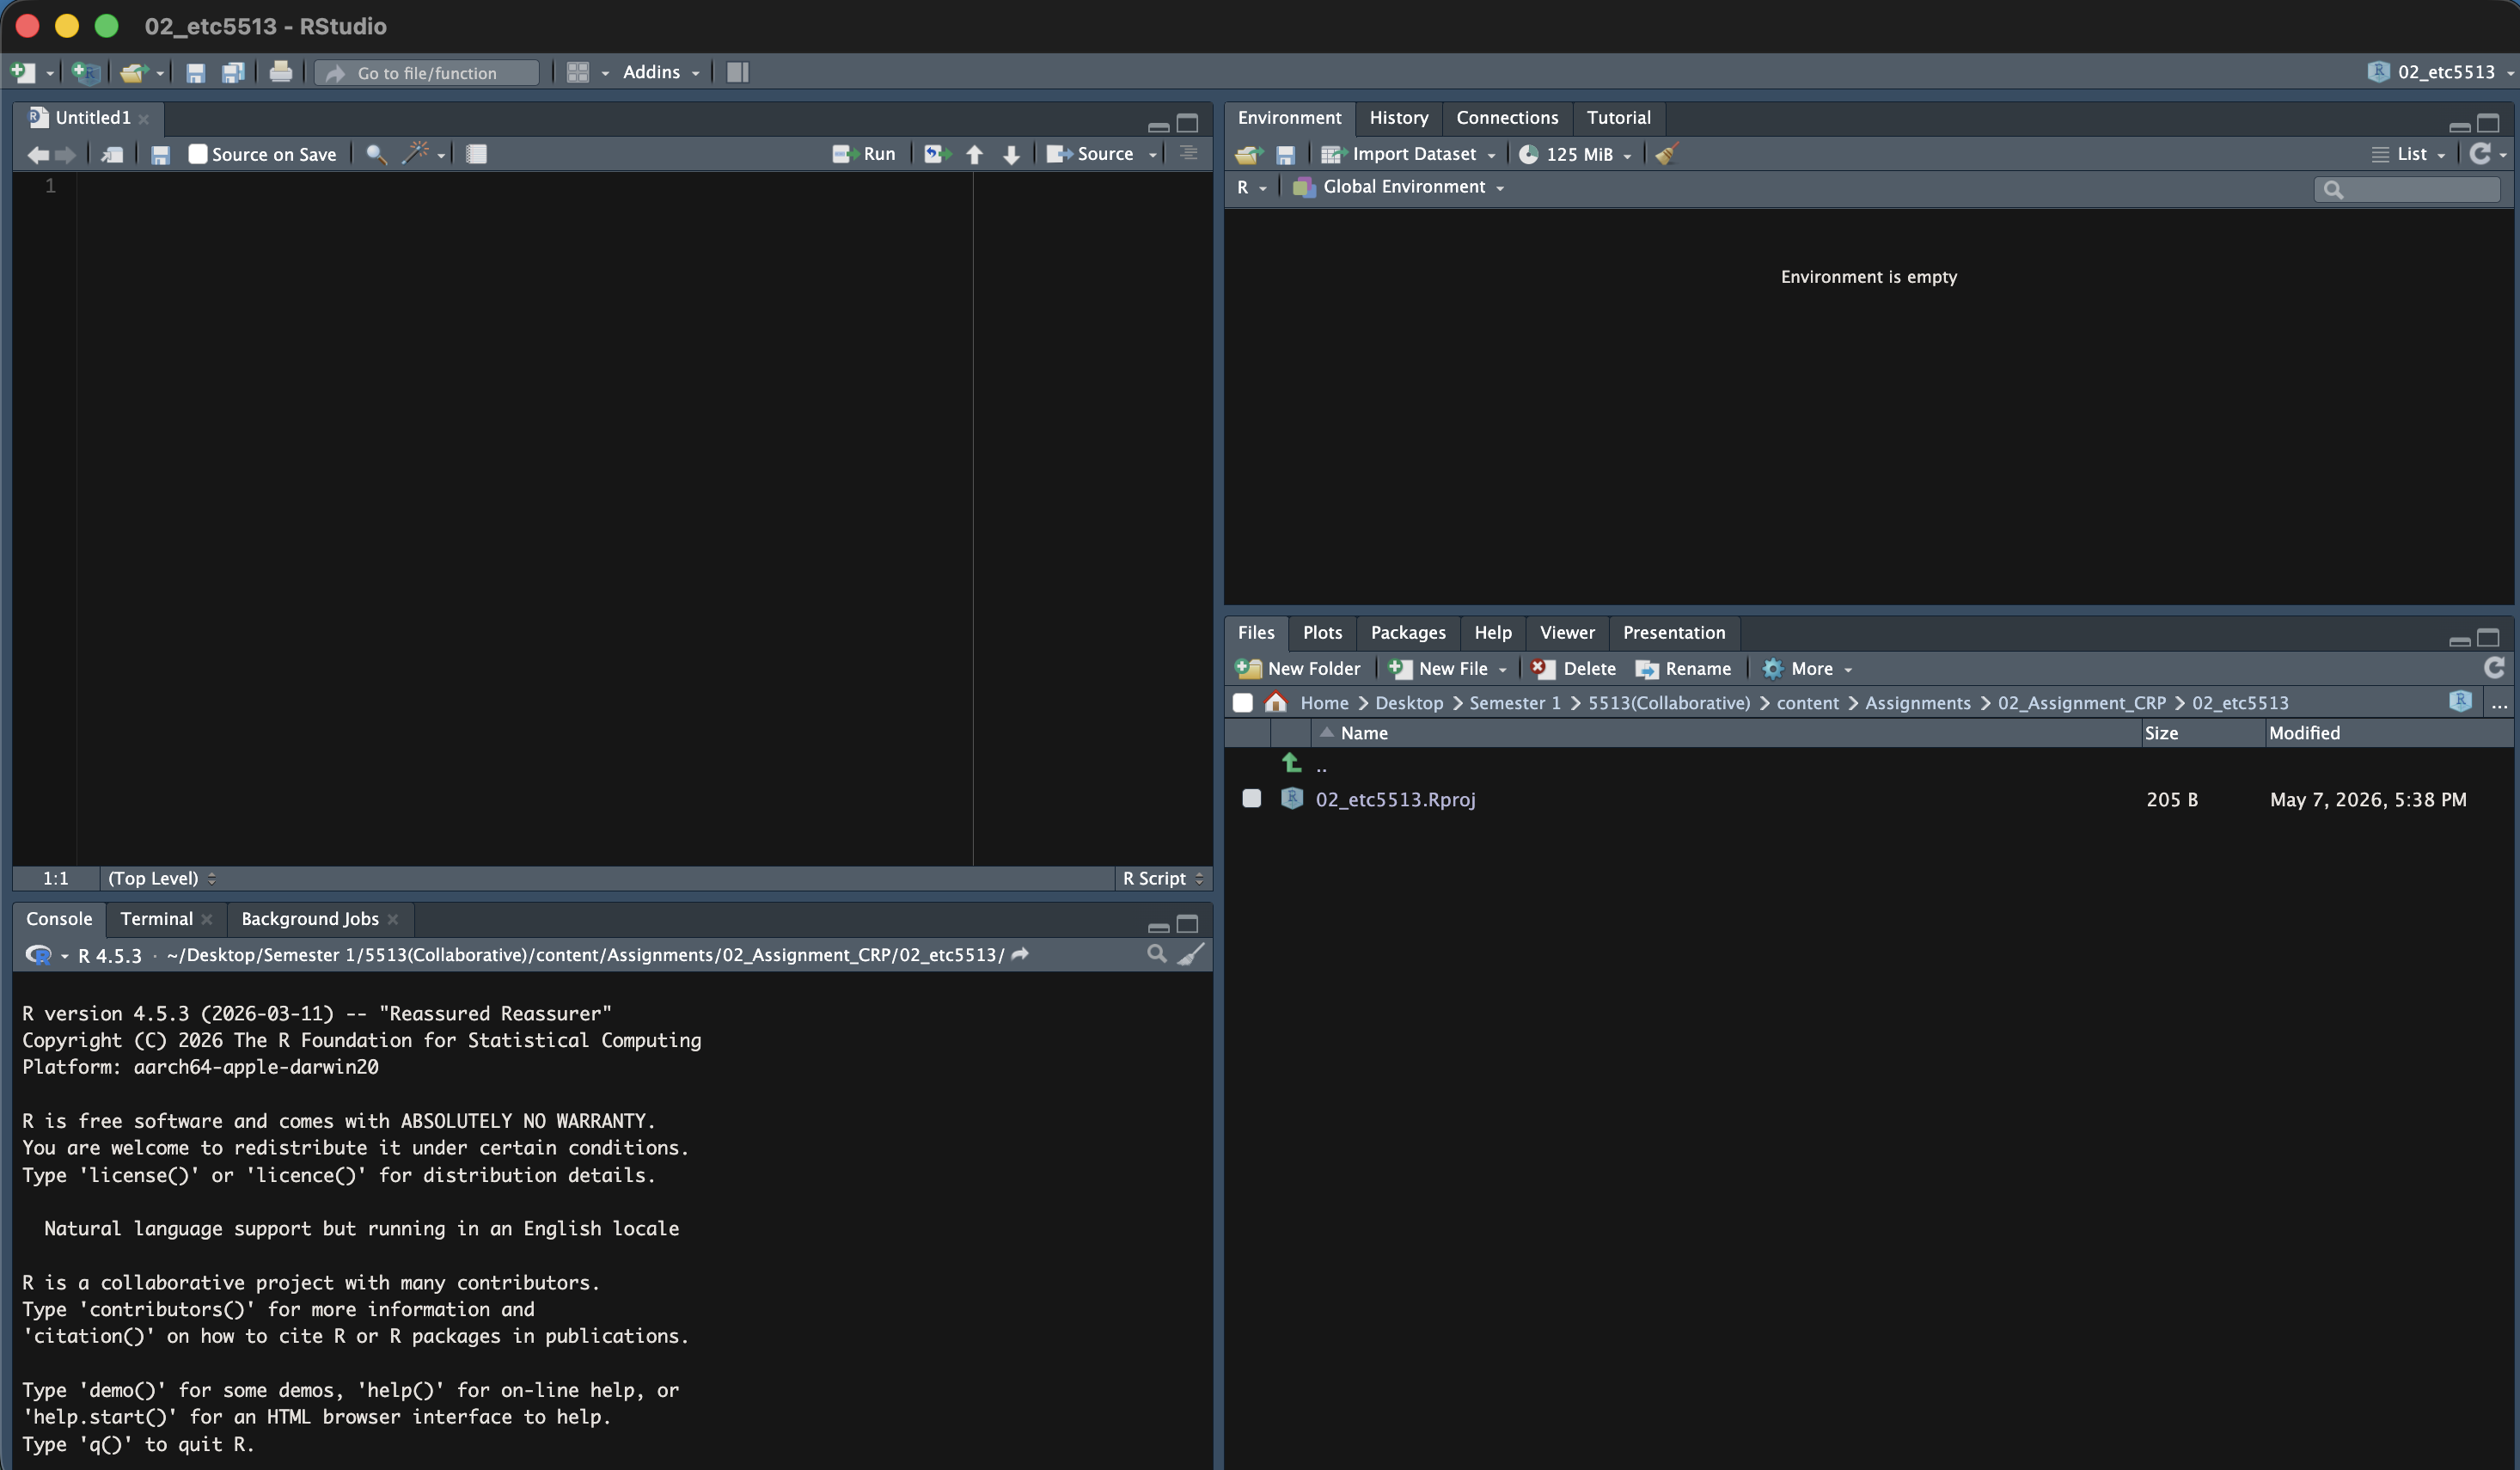
\includegraphics[keepaspectratio]{images/clipboard-759875795.png}}

Part B: Create the \texttt{example.qmd} file

A \texttt{.qmd} file is a \textbf{Quarto Markdown} file --- it lets you
mix plain text, formatting, and R code chunks, then render it all into a
nice HTML (or PDF, etc.) document.

\begin{enumerate}
\def\labelenumi{\arabic{enumi}.}
\item
  Go to \textbf{File → New File → Quarto Document\ldots{}}
\item
  A dialog appears:

  \begin{itemize}
  \item
    \textbf{Title:} type something like ``Assignment\_02\_Example''
  \item
    \textbf{Author:} ``Tushar Dhanorkar''
  \item
    Make sure \textbf{HTML} is selected as the output format
  \end{itemize}
\item
  Click \textbf{Create}
\item
  Your file will have a YAML header at the top (between the
  \texttt{-\/-\/-} lines) and some default content. You can simplify it
  to look like this:
\end{enumerate}

Part C: Render (Knit) the file to HTML

\begin{enumerate}
\def\labelenumi{\arabic{enumi}.}
\item
  The YAML header controls the document settings. The
  \texttt{\#\#\ Introduction} is a heading. The
  \texttt{\textasciigrave{}\textasciigrave{}\textasciigrave{}\{r\}}
  block is an R code chunk --- it will run the R code and show the
  output in the rendered document.
\item
  Rendering'' means Quarto takes your \texttt{.qmd} file, runs all the R
  code, and produces a finished HTML file.
\item
  Click the \textbf{Render} button at the top of the editor.
\end{enumerate}

\pandocbounded{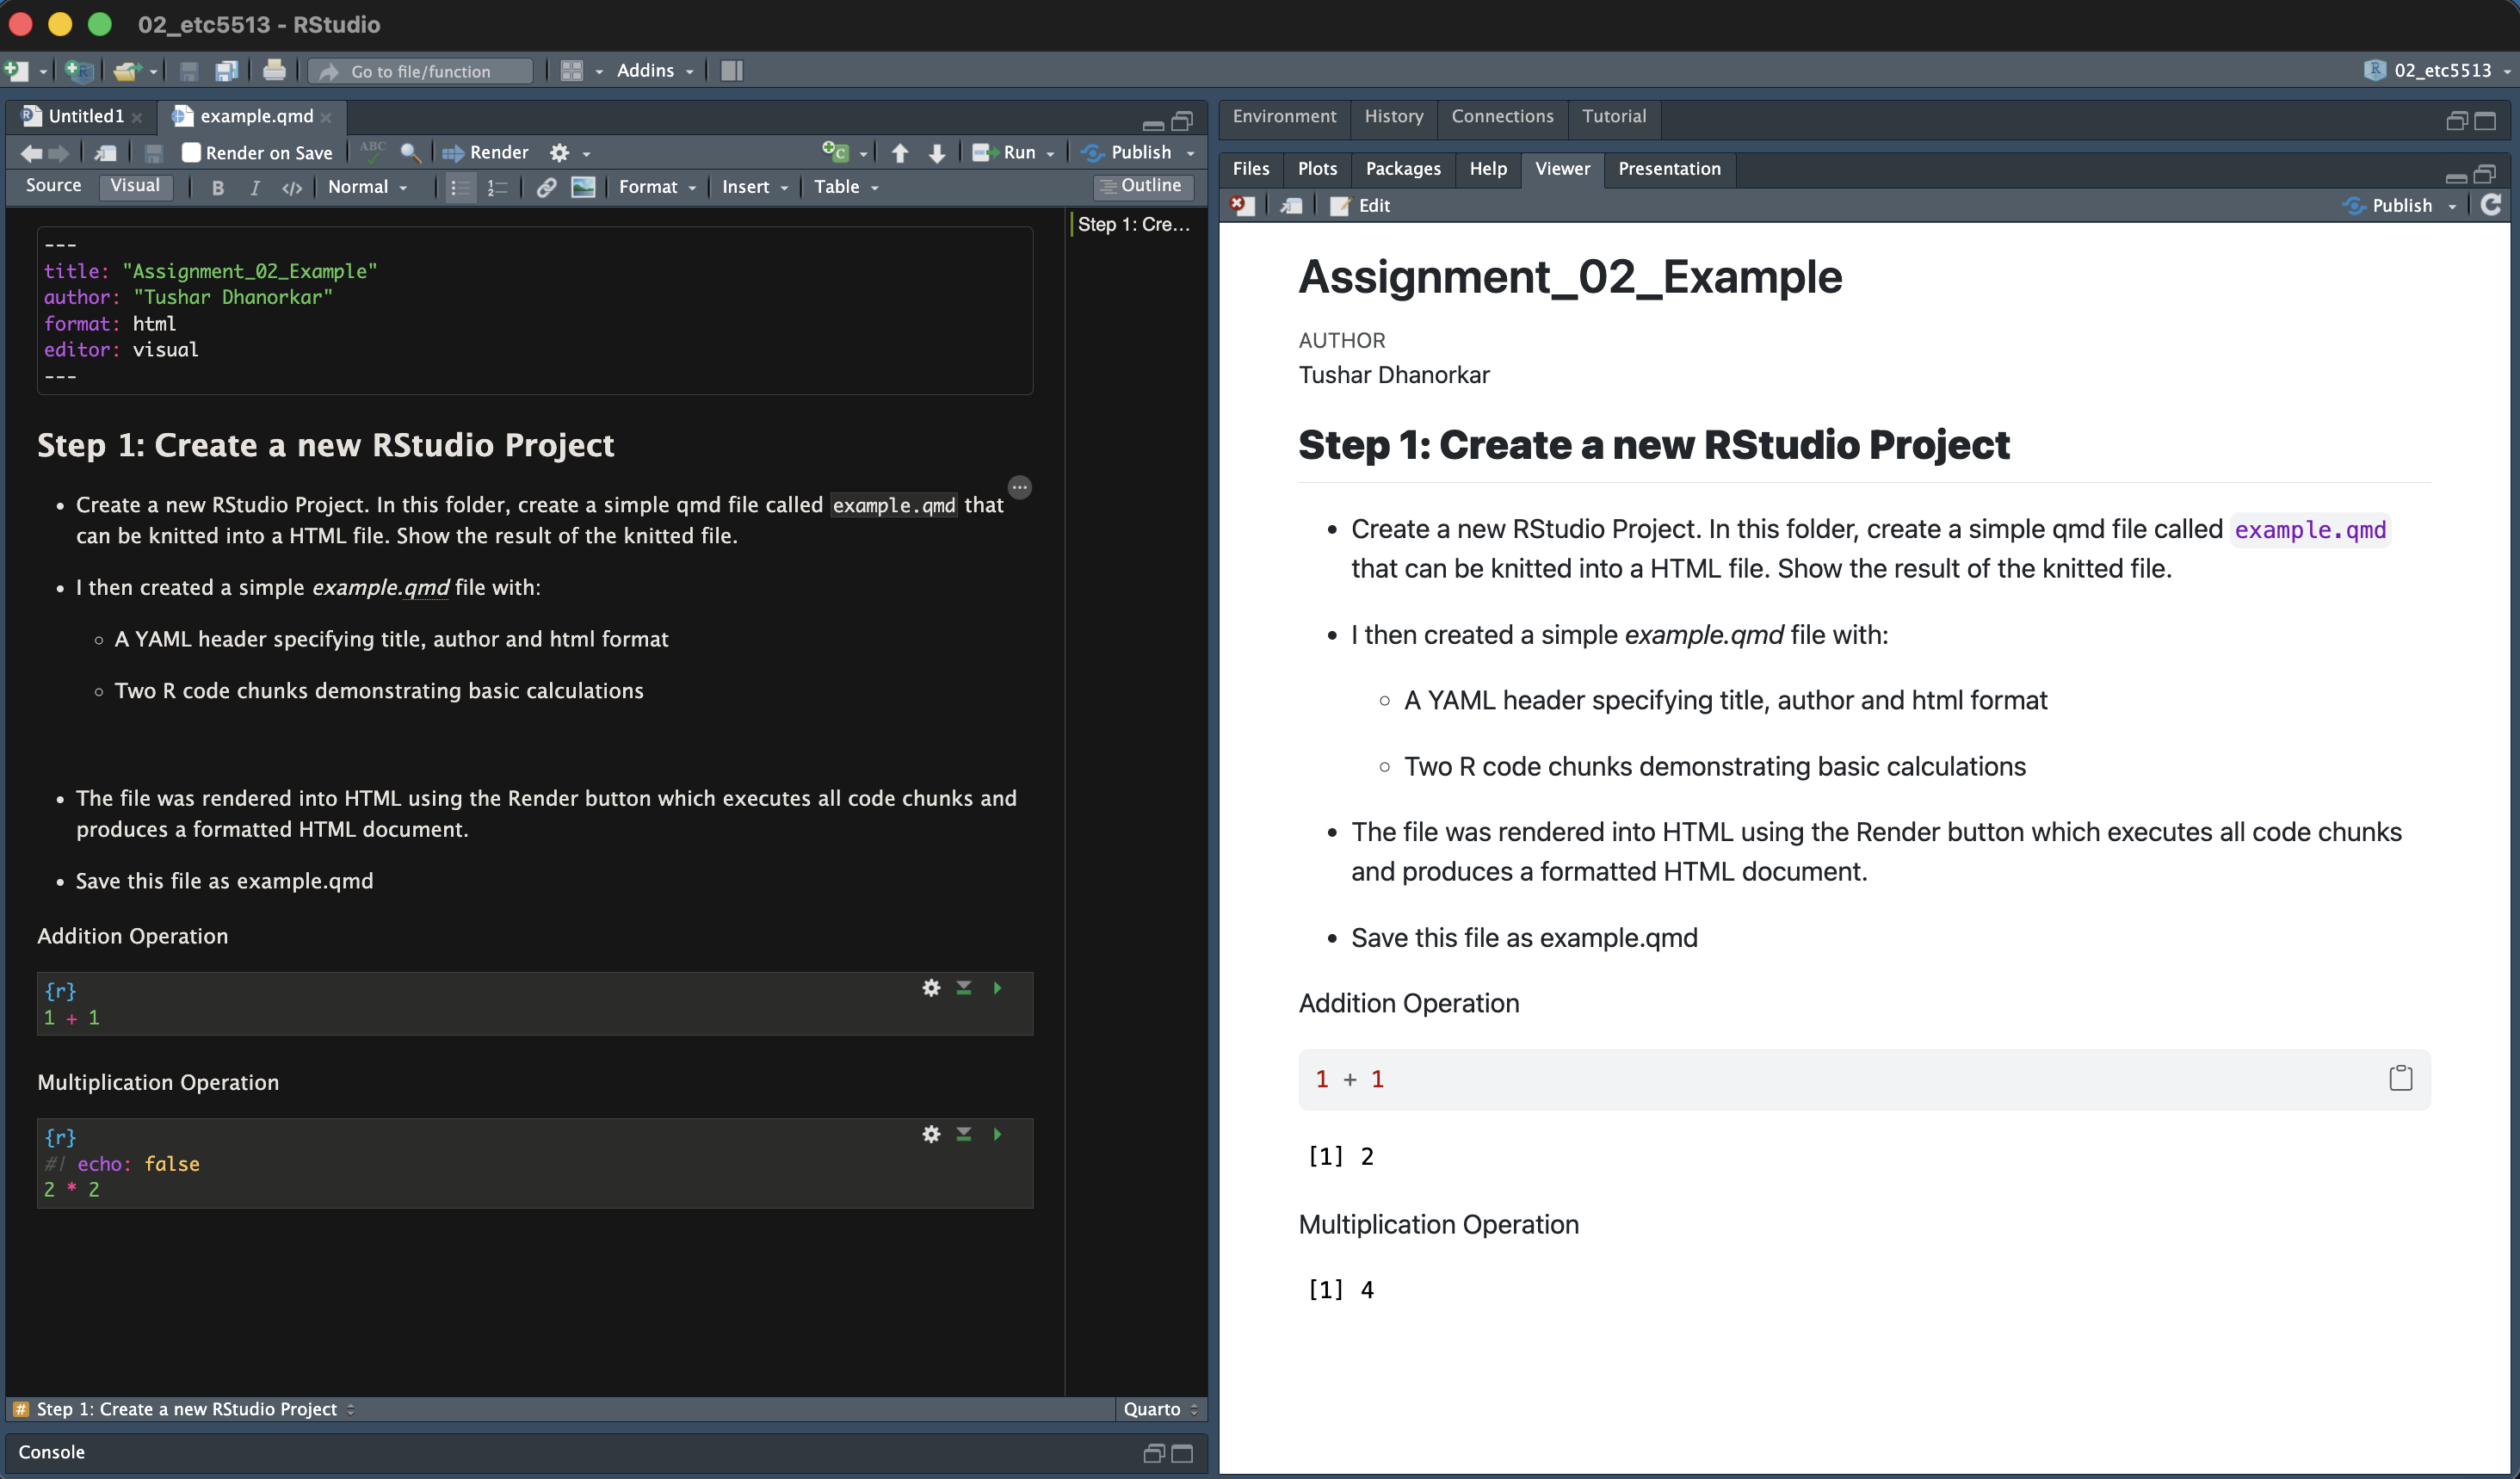
\includegraphics[keepaspectratio]{images/clipboard-2708816945.png}}

\paragraph{\texorpdfstring{\textbf{Step 2: Initialise Git and push to
GitHub}}{Step 2: Initialise Git and push to GitHub}}\label{step-2-initialise-git-and-push-to-github}

\begin{enumerate}
\def\labelenumi{\arabic{enumi}.}
\item
  What you need before starting:

  \begin{itemize}
  \item
    \textbf{Git installed} on your computer (type
    \texttt{git\ -\/-version} in your terminal to check)
  \item
    A \textbf{GitHub account} at github.com
  \item
    Git configured with your name and email (only needs to be done
    once):
  \end{itemize}
\item
  Open the Terminal and navigate to your project folder

  \begin{itemize}
  \item
    Go to \textbf{Tools → Terminal → New Terminal}
  \item
    Or click the \textbf{Terminal} tab next to Console
  \end{itemize}
\item
  You need to make sure you're inside your project folder. Since RStudio
  Projects automatically set the working directory, you should already
  be there. Confirm it by typing:
\item
  pwd

  \begin{itemize}
  \tightlist
  \item
    This prints your current directory. It should end with
    \texttt{/02\_etc5513}
  \end{itemize}
\item
  git init

  \begin{itemize}
  \tightlist
  \item
    This creates a hidden \texttt{.git} folder inside your project
    folder. That folder is what makes it a Git repository --- it stores
    all version history.
  \end{itemize}
\item
  git status

  \begin{itemize}
  \tightlist
  \item
    You'll see \texttt{example.qmd,\ example.html\ ,\ images/\ ,\ etc}as
    untracked files.
  \end{itemize}
\item
  git add .

  \begin{itemize}
  \tightlist
  \item
    \textbf{stage} all of them (tell Git you want to include them in the
    next commit), The \texttt{.} means ``add everything in this folder''
  \end{itemize}
\item
  \texttt{git\ status} - Files should now show in green under ``Changes
  to be committed''git commit -m ``First commit add example.qmd and
  project files''
\end{enumerate}

Part B: Create a GitHub repository

\begin{enumerate}
\def\labelenumi{\arabic{enumi}.}
\item
  Go to \textbf{github.com} and log in

  \begin{itemize}
  \item
    \textbf{Repository name:} \texttt{02\_etc5513}
  \item
    Click \textbf{Create repository}
  \end{itemize}
\end{enumerate}

\pandocbounded{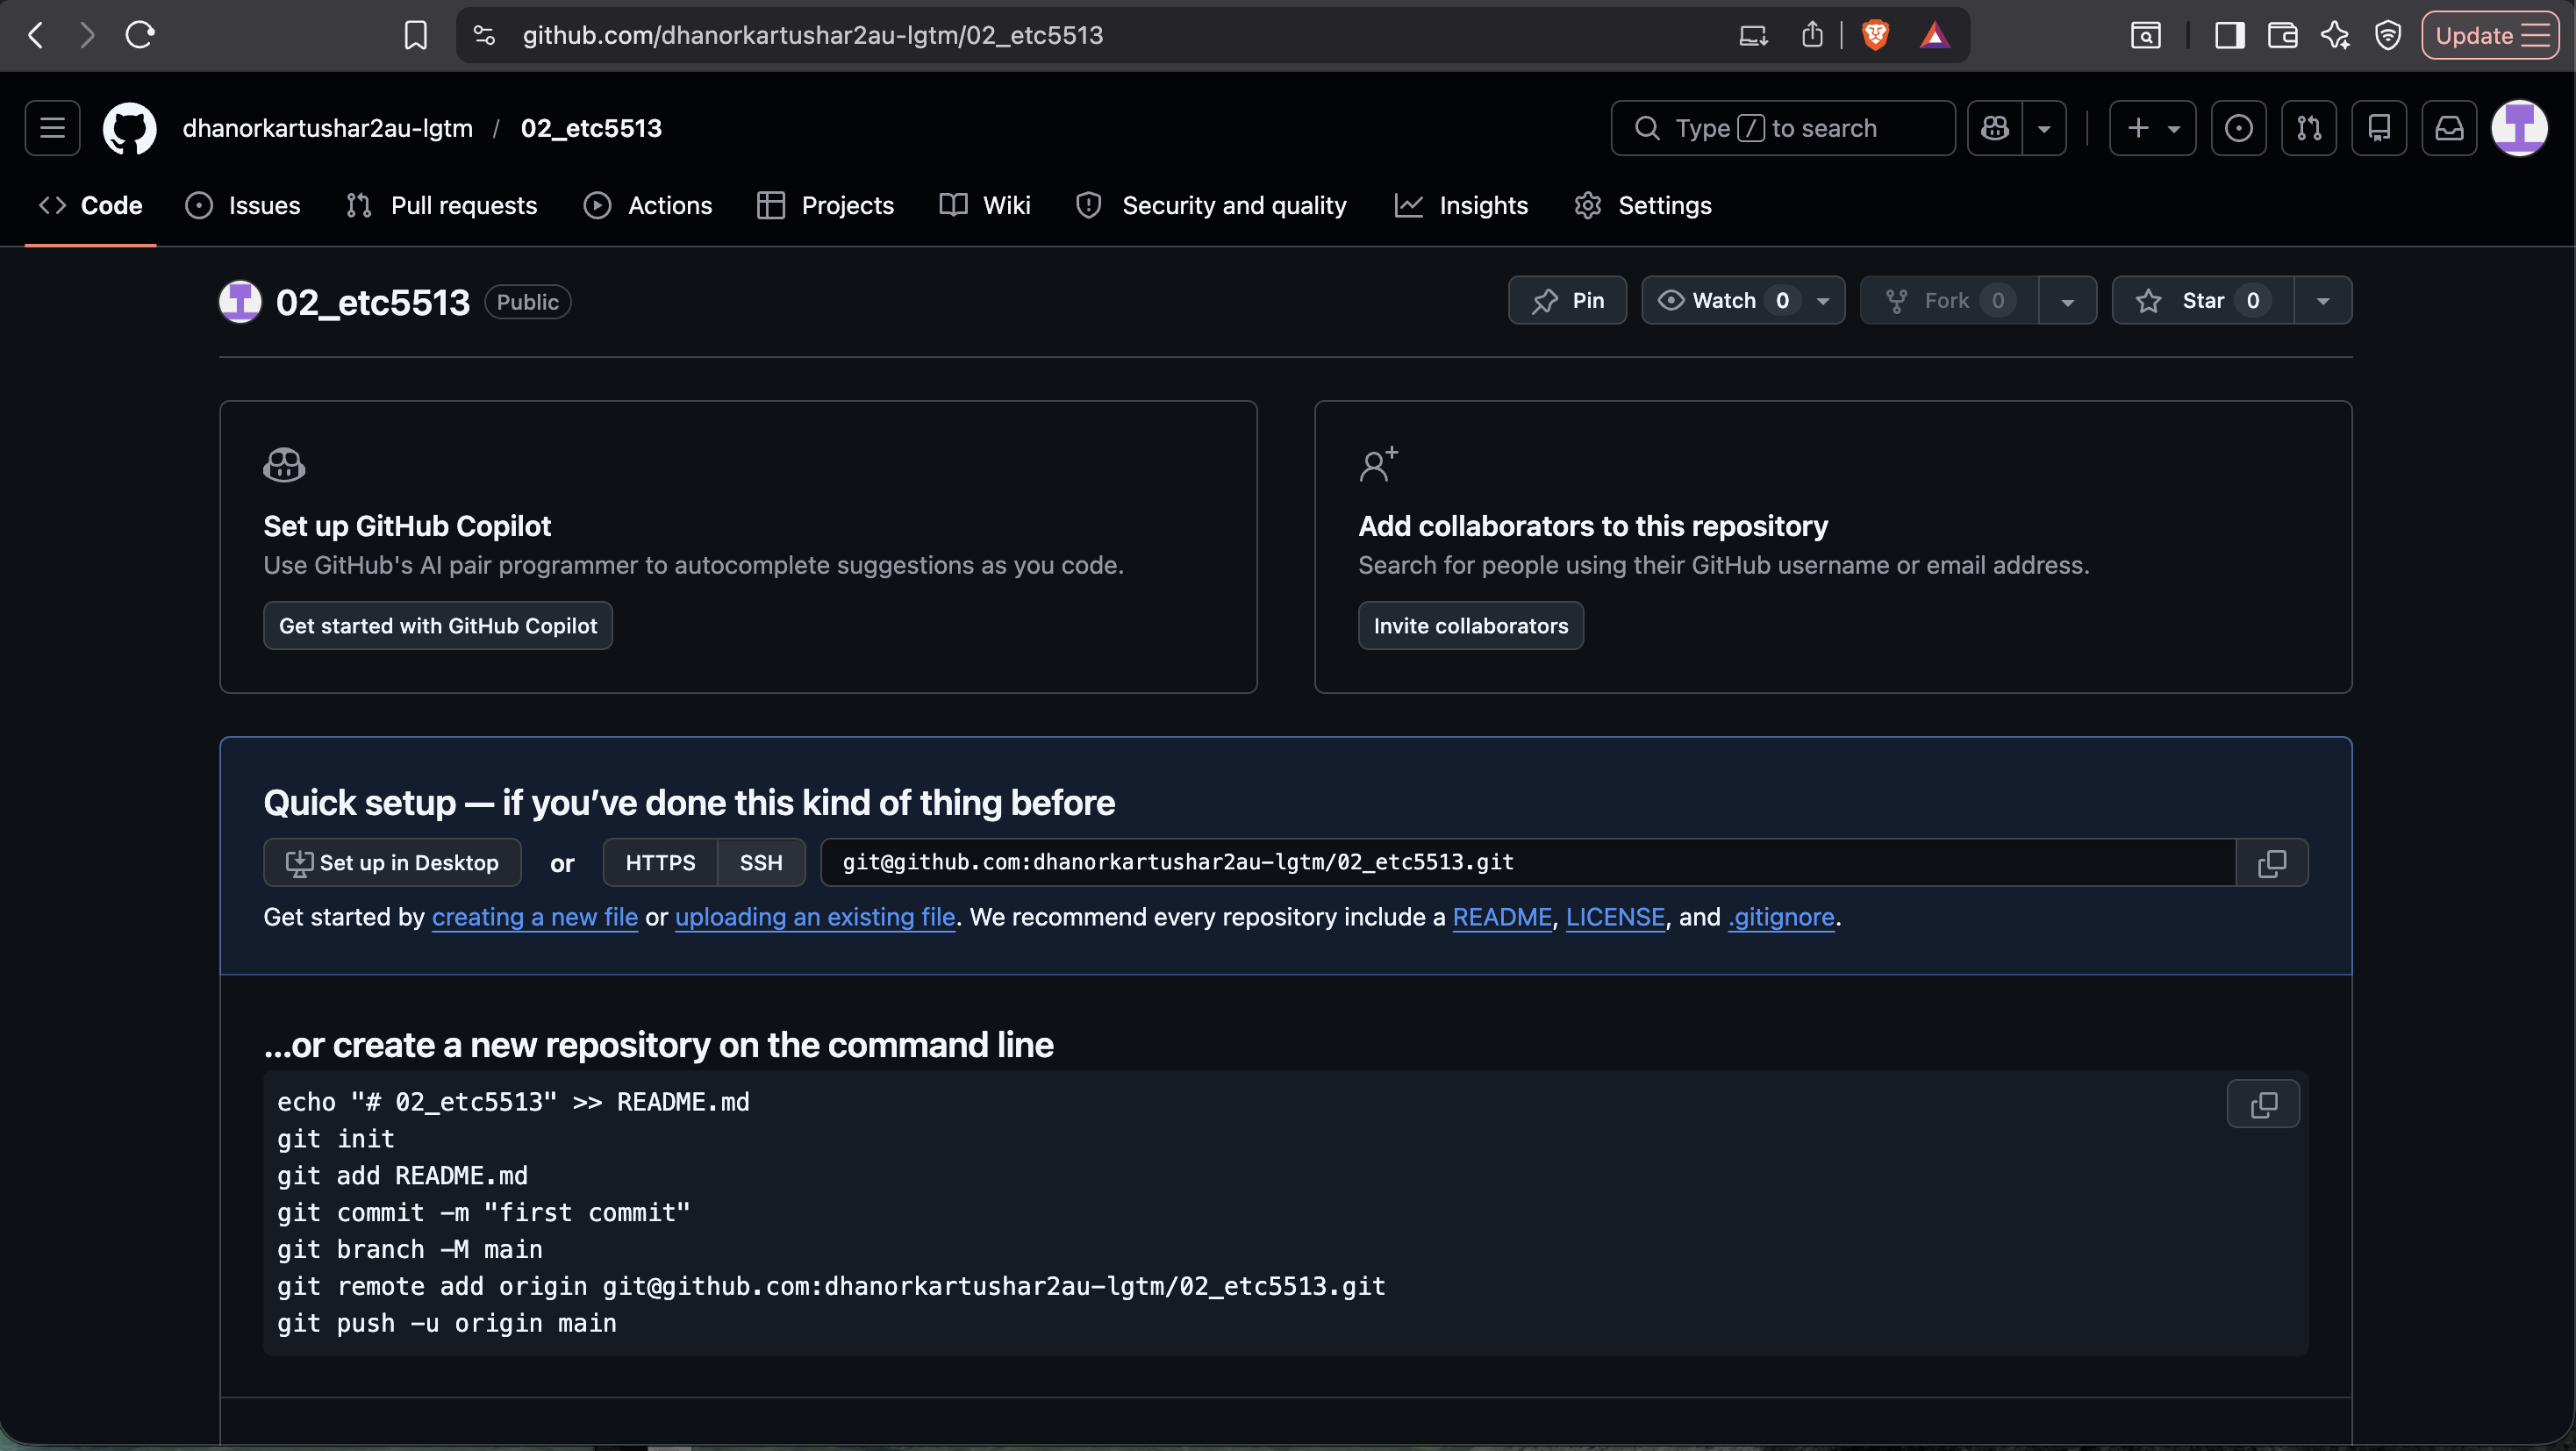
\includegraphics[keepaspectratio]{images/clipboard-2675037616.png}}

Part C: Connect your local repo to GitHub and push

\pandocbounded{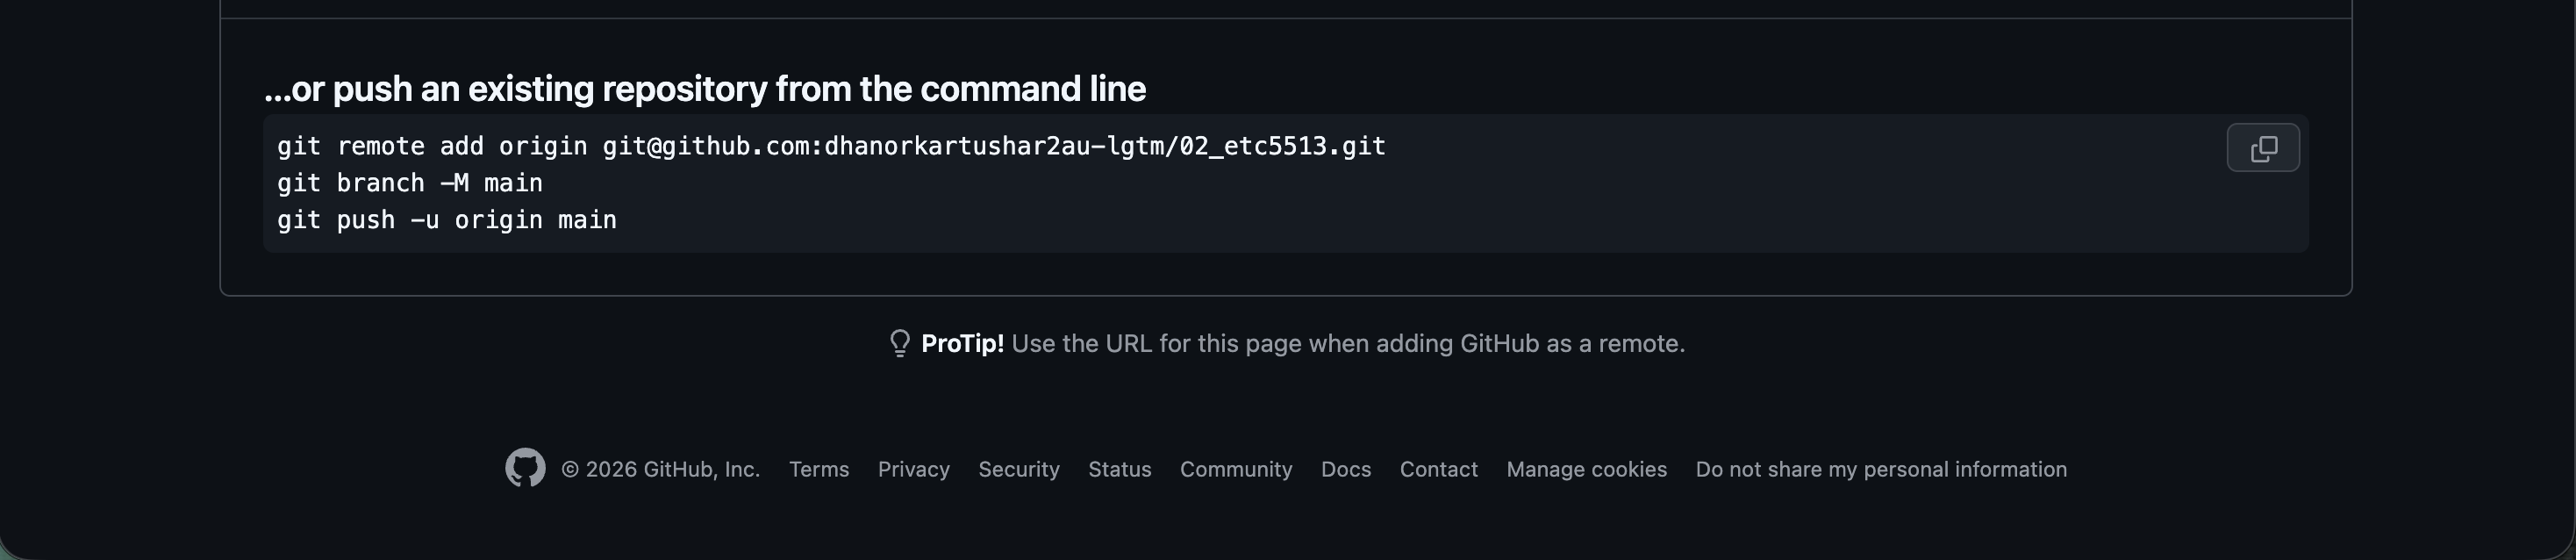
\includegraphics[keepaspectratio]{images/clipboard-185792810.png}}

\begin{itemize}
\item
  \texttt{git\ remote\ add\ origin\ git@github.com:dhanorkartushar2au-lgtm/02\_etc5513.git}

  \begin{itemize}
  \tightlist
  \item
    This command \textbf{links your local repository to your GitHub
    repository -} Adding new remote with nickname as Origin to the
    address of our Github repository i.e by SSH
  \end{itemize}
\item
  \texttt{git\ branch\ -M\ main}

  \begin{itemize}
  \item
    This command \textbf{renames your current branch to \texttt{main}}
  \item
    \texttt{git\ branch} --- used to manage branches , \texttt{-M} ---
    means ``force rename'',\texttt{main} --- the new name for your
    branch
  \end{itemize}
\item
  git push -u origin main

  \begin{itemize}
  \tightlist
  \item
    This command \textbf{uploads your local commits to GitHub}.
  \end{itemize}
\end{itemize}

\pandocbounded{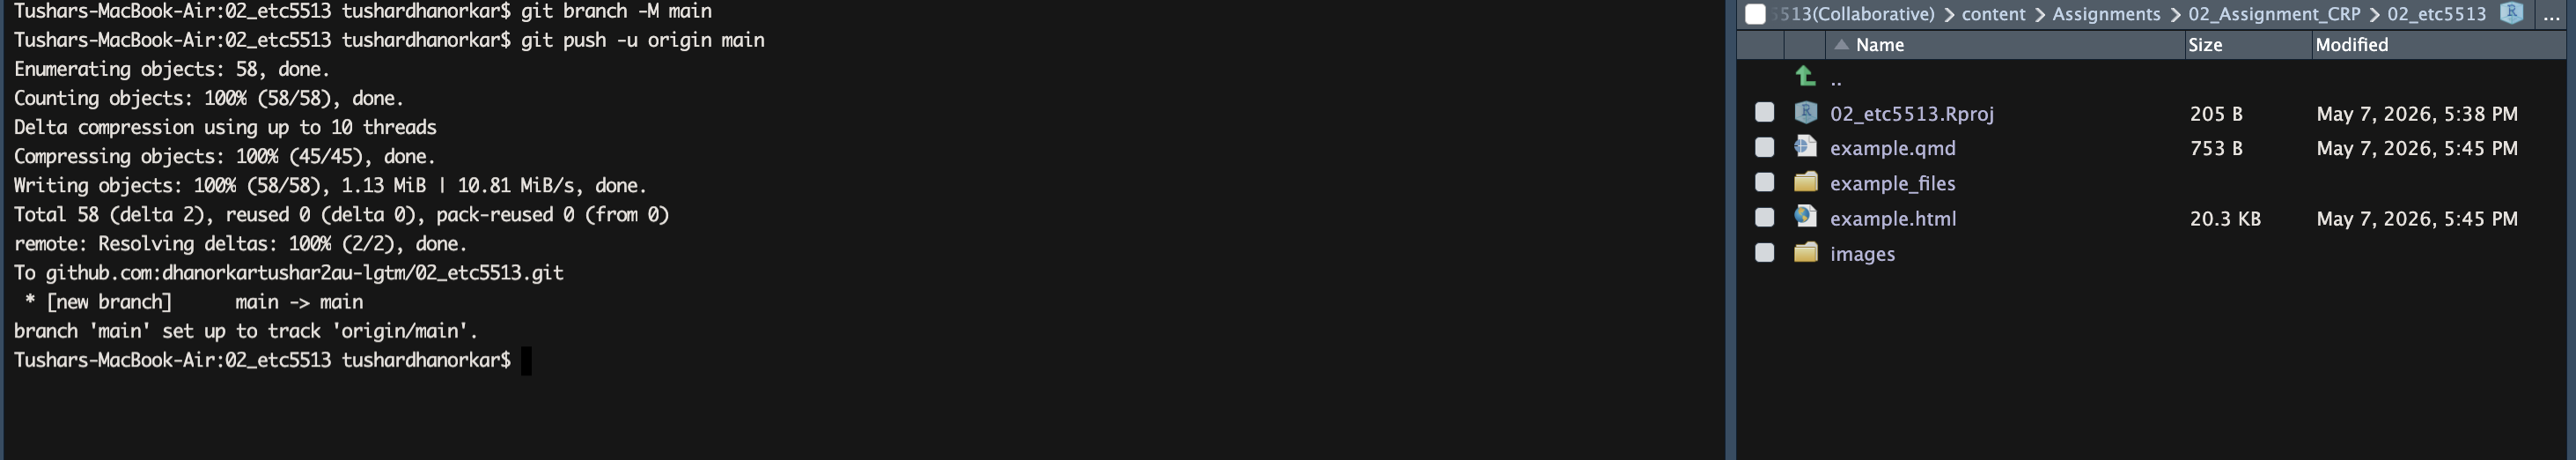
\includegraphics[keepaspectratio]{images/clipboard-1623071871.png}}

\paragraph{\texorpdfstring{\textbf{Step 3:} Create \texttt{testbranch},
Modify \texttt{example.qmd}, and
Push:}{Step 3: Create testbranch, Modify example.qmd, and Push:}}\label{step-3-create-testbranch-modify-example.qmd-and-push}

When you create a branch, you get an exact copy of your current files to
work on freely --- without affecting the \texttt{main} branch. This is
useful when you want to try something new or make changes without
breaking your working code

Part A: Create and switch to \texttt{testbranch}

\begin{enumerate}
\def\labelenumi{\arabic{enumi}.}
\item
  \texttt{git\ checkout\ -b\ testbranch} expected output: Switched to a
  new branch `testbranch'

  \begin{itemize}
  \item
    \texttt{git\ checkout} --- switches branches,\texttt{-b} --- means
    ``create this branch if it doesn't exist'',\texttt{testbranch} ---
    the name of the new branch
  \item
    \texttt{git\ branch} - This lists all branches. The one with a
    \texttt{*}
  \end{itemize}
\end{enumerate}

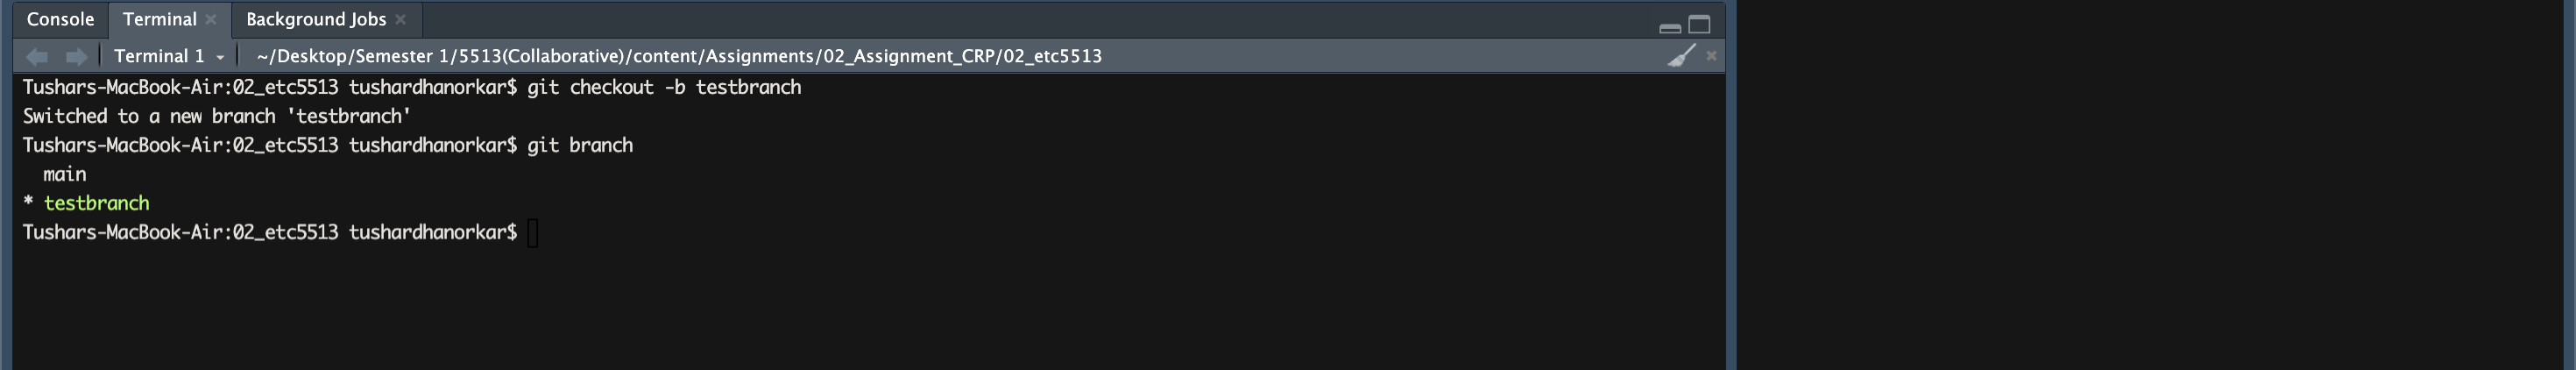
\includegraphics[width=37.69792in,height=\textheight,keepaspectratio]{images/clipboard-388725881.png}

Part A: Create and switch to \texttt{testbranch} and push

\begin{enumerate}
\def\labelenumi{\arabic{enumi}.}
\item
  Modify \texttt{example.qmd}

  \begin{itemize}
  \item
    Open \texttt{example.qmd} in RStudio and make a change to it. For
    example, add a new section

\begin{Shaded}
\begin{Highlighting}[]
\NormalTok{x }\OtherTok{\textless{}{-}} \FunctionTok{c}\NormalTok{(}\DecValTok{10}\NormalTok{, }\DecValTok{20}\NormalTok{, }\DecValTok{30}\NormalTok{, }\DecValTok{40}\NormalTok{, }\DecValTok{50}\NormalTok{)}
\FunctionTok{mean}\NormalTok{(x)}
\end{Highlighting}
\end{Shaded}

\begin{verbatim}
[1] 30
\end{verbatim}
  \end{itemize}
\item
  \texttt{git\ status} - Check what changed, You'll see
  \texttt{example.qmd} listed as modified
\item
  \texttt{git\ add\ .} - Stage all modified files
\item
  \texttt{git\ commit\ -m\ "Add\ new\ section\ to\ example.qmd\ on\ testbranch"}
  - Commit with a clear message
\item
  \texttt{git\ push\ -u\ origin\ testbranch} - This pushes the branch to
  GitHub. The \texttt{-u} sets the upstream so future pushes on this
  branch only need \texttt{git\ push}
\end{enumerate}

\pandocbounded{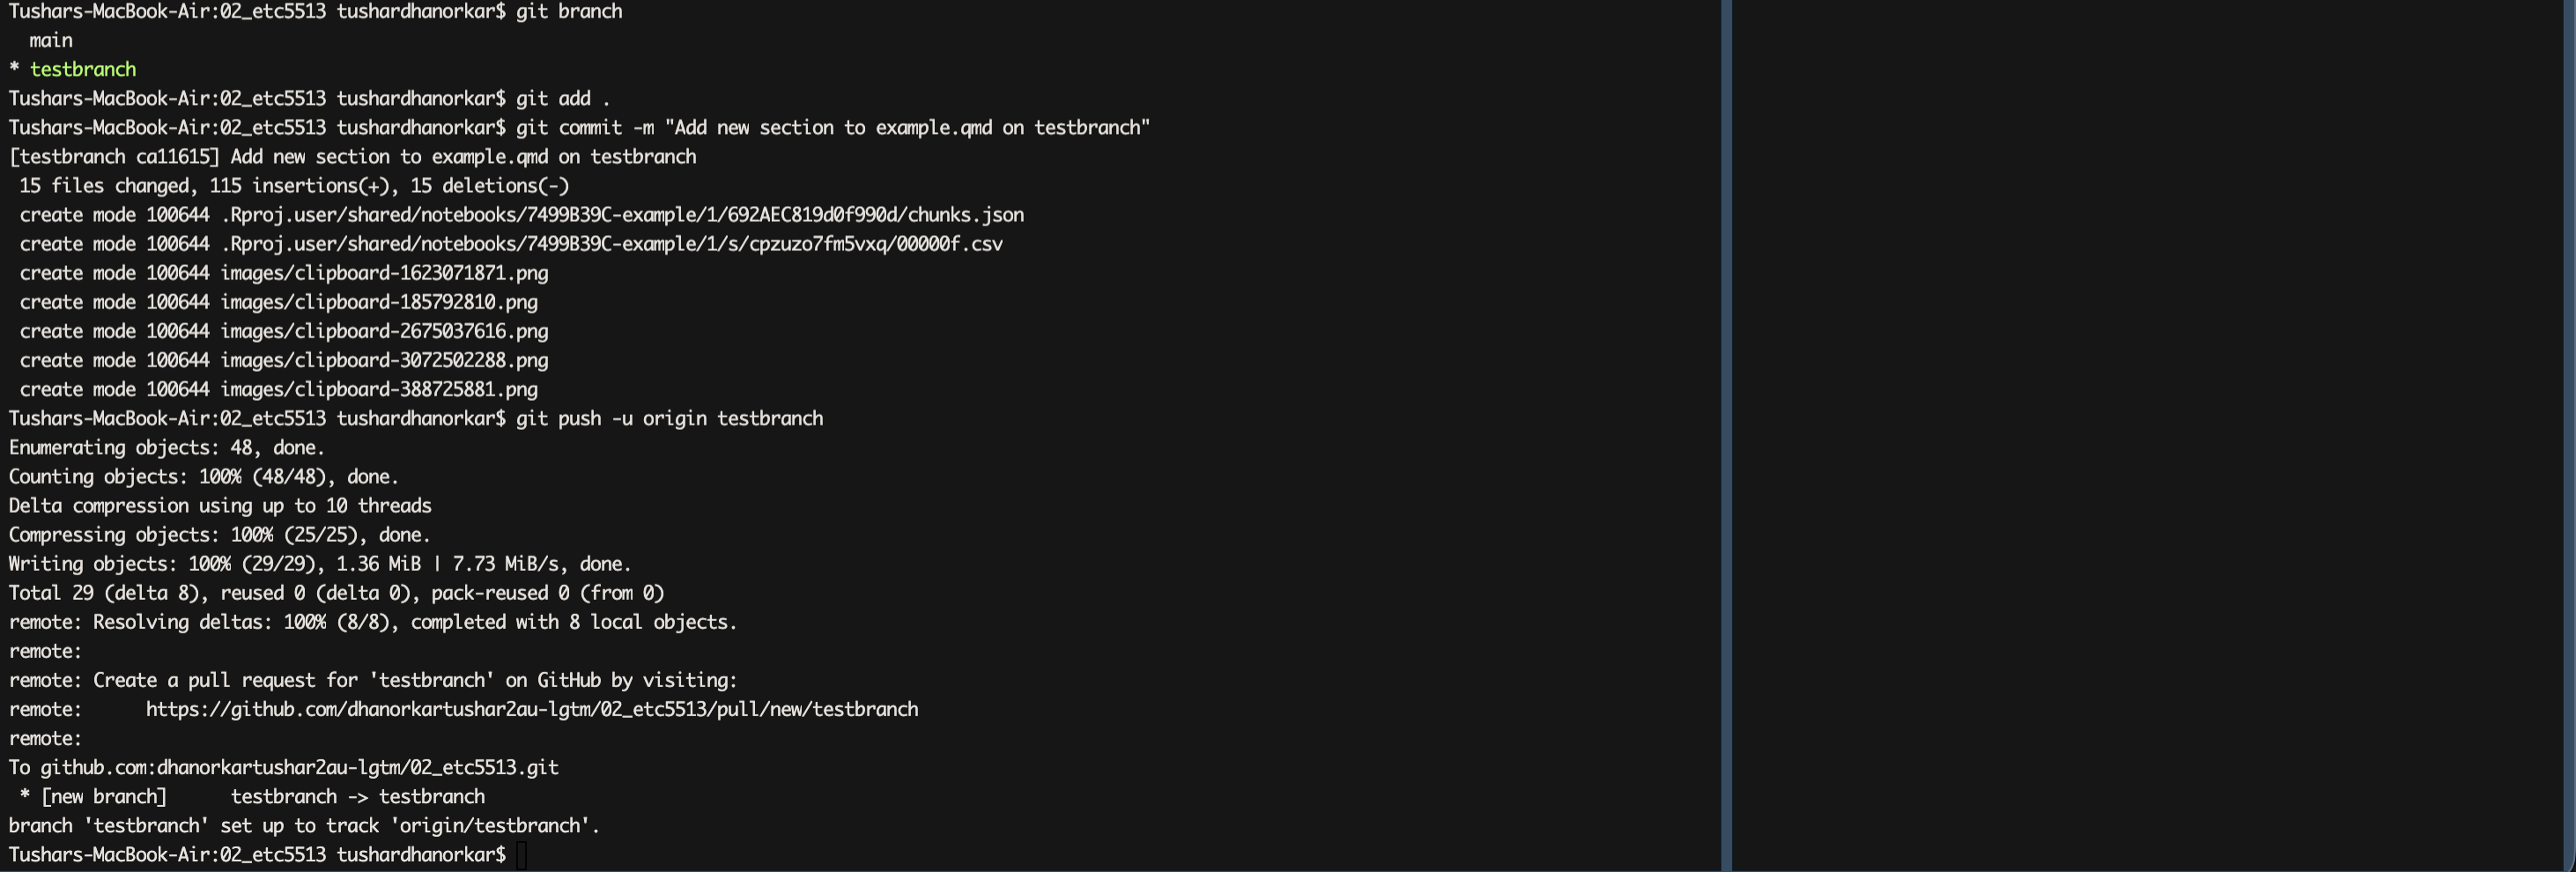
\includegraphics[keepaspectratio]{images/clipboard-4171620953.png}}

When we ran \texttt{git\ add\ .} AND
\texttt{git\ commit\ -m\ "Add\ new\ section\ to\ example.qmd\ on\ testbranch"}
changes were saved to our local repository.

When we ran \texttt{git\ push\ -u\ origin\ testbranch} Those same
changes were uploaded to \textbf{GitHub.}

\paragraph{\texorpdfstring{\textbf{Step 4:} Create \texttt{data/}
Folder, Add Assignment 1 Data, and Amend the Previous
Commit}{Step 4: Create data/ Folder, Add Assignment 1 Data, and Amend the Previous Commit}}\label{step-4-create-data-folder-add-assignment-1-data-and-amend-the-previous-commit}

Amending means \textbf{modifying the most recent commit} --- instead of
creating a brand new commit, you update the last one to include
something you forgot.

So in this case, we are going back to last commit in branch testbranch
and saying that ``we wanted to add data folder''

\begin{enumerate}
\def\labelenumi{\arabic{enumi}.}
\item
  Ensure that we are on testbranch

  \begin{itemize}
  \tightlist
  \item
    \texttt{git\ checkout\ testbranch} - switch to testbranch we in case
    we are not in
  \end{itemize}
\item
  Create the \texttt{data/} folder and add your Assignment 1 data
\item
  \texttt{mkdir\ data}

  \begin{itemize}
  \tightlist
  \item
    This creates a folder called \texttt{data} inside your project.
  \end{itemize}
\item
  \texttt{git\ status} we can see that data folder is unstage

  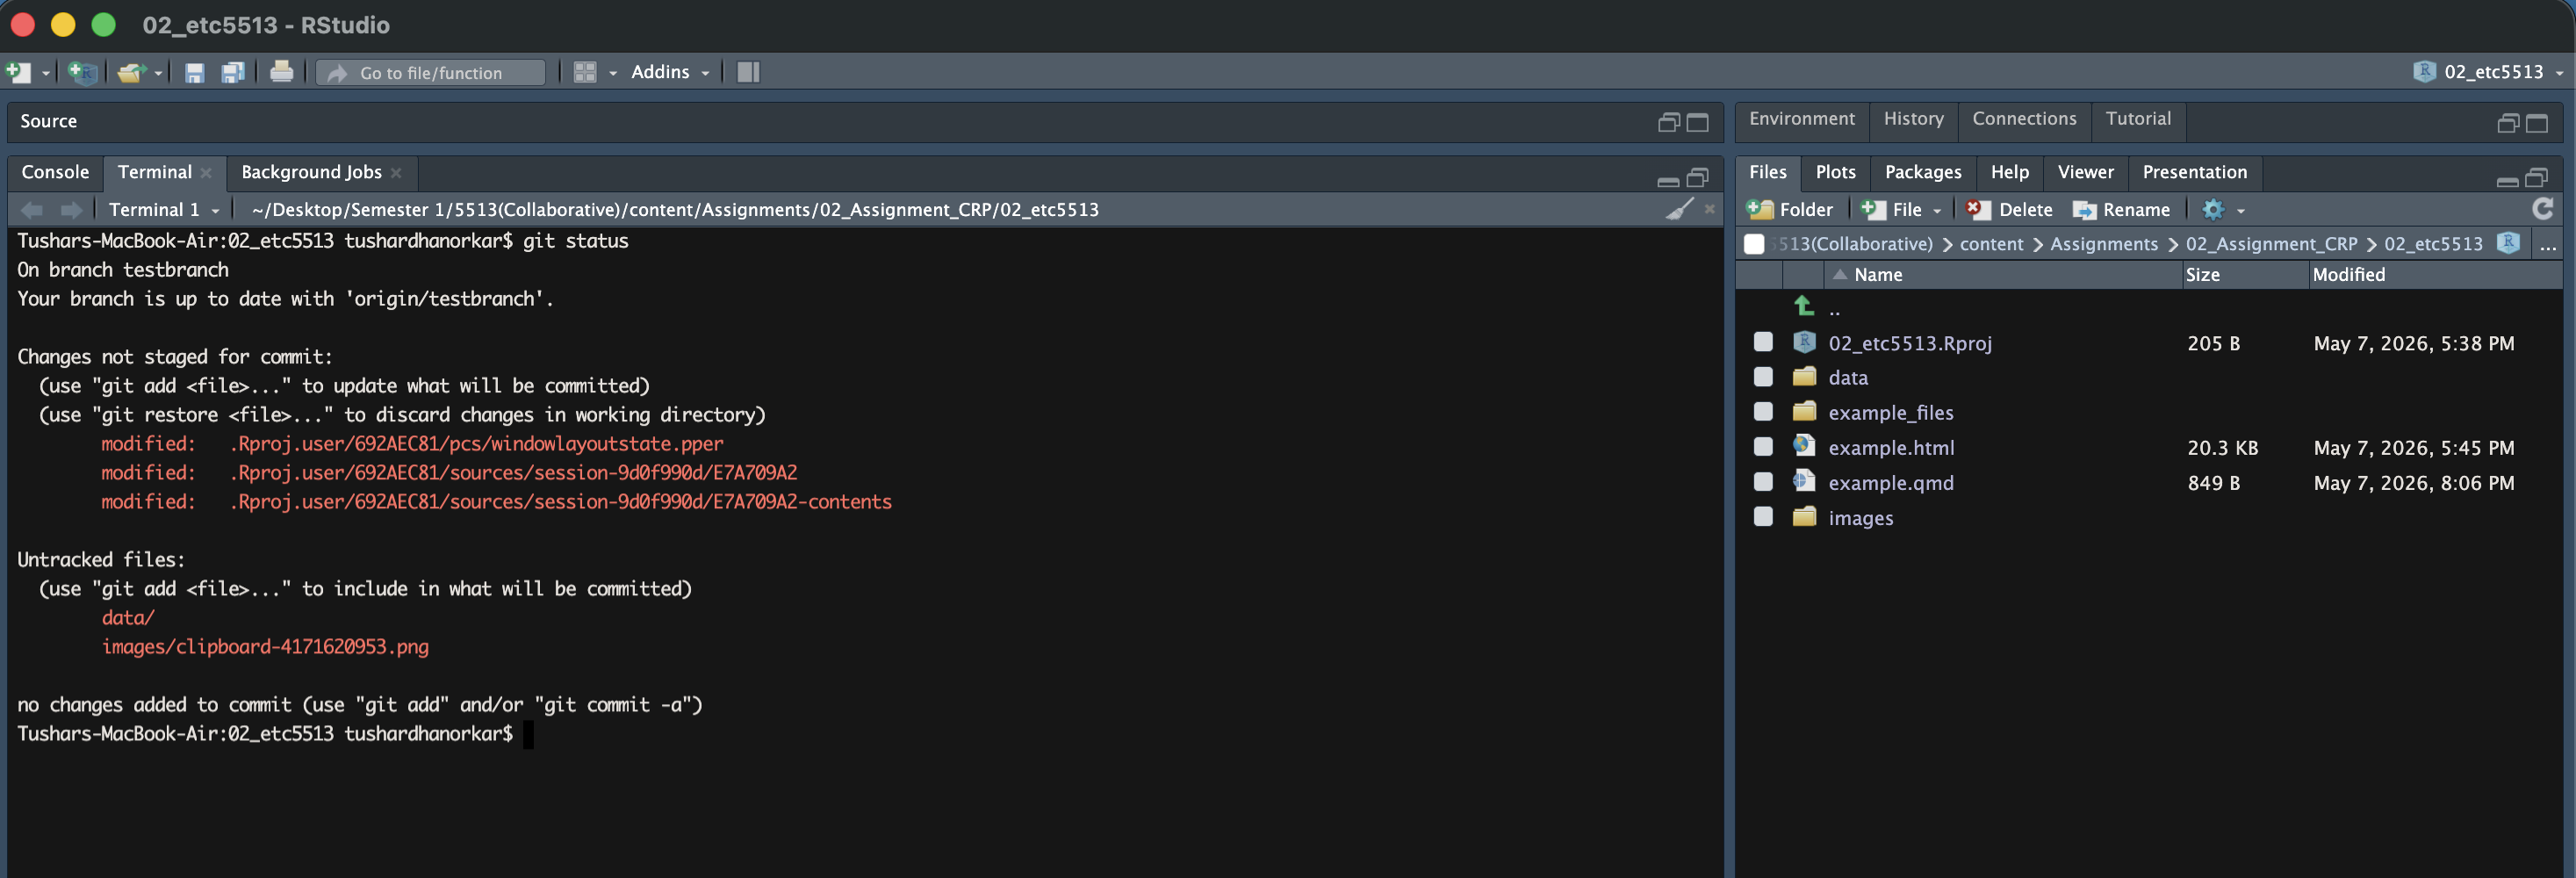
\includegraphics[width=7.35417in,height=\textheight,keepaspectratio]{images/clipboard-3041359356.png}
\item
  \texttt{git\ add\ data/} Stage the data folder
\item
  \texttt{git\ status} Now check the status and the data file(s) listed
  as staged under ``Changes to be committed''

  \pandocbounded{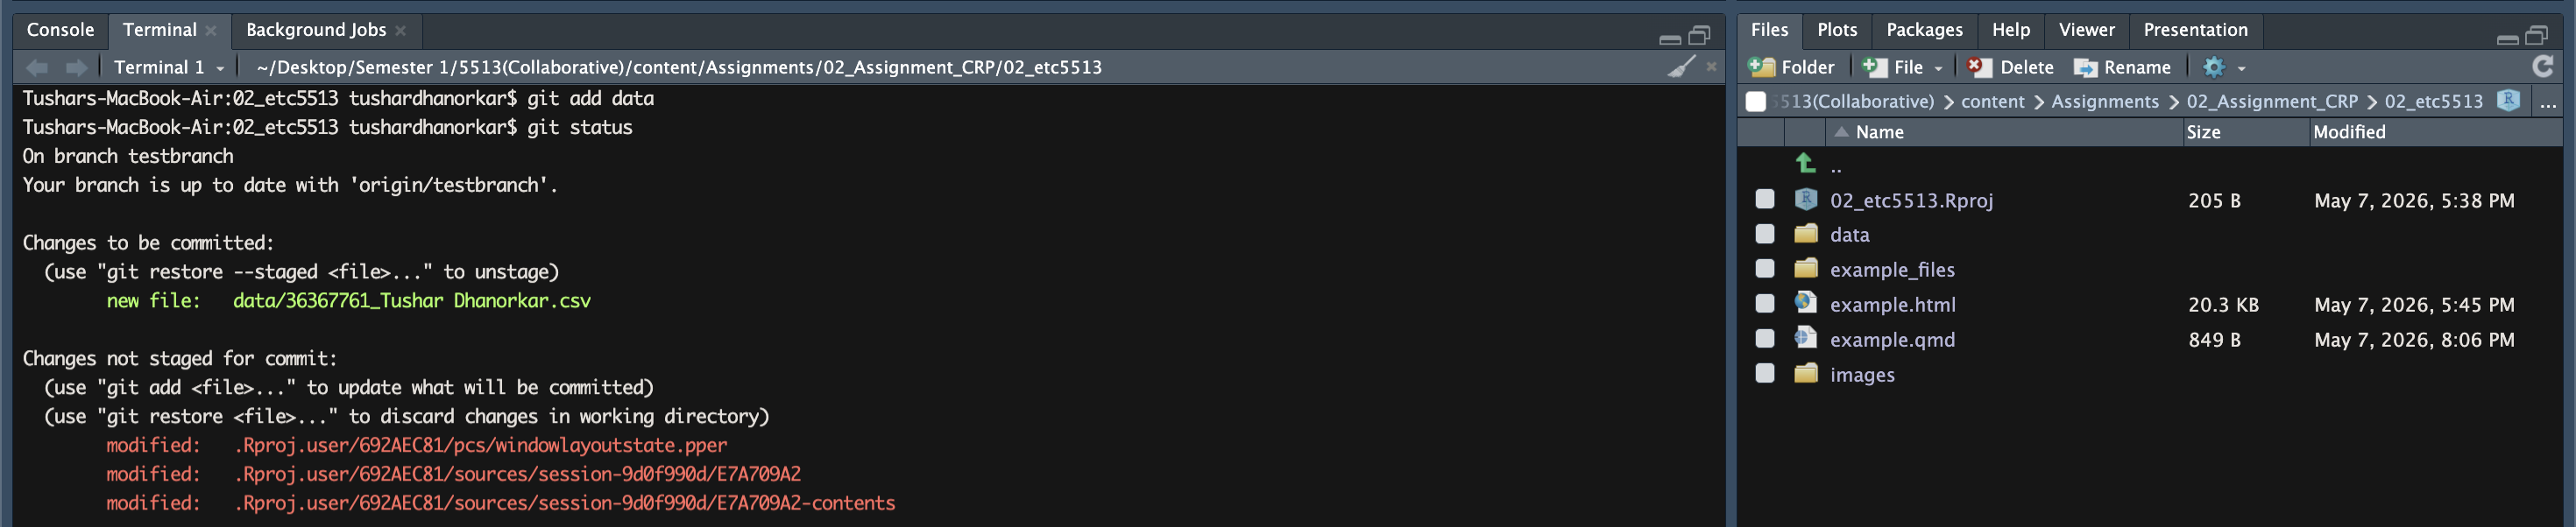
\includegraphics[keepaspectratio]{images/clipboard-2936962398.png}}
\item
  \texttt{git\ commit\ -\/-amend\ -m\ "Adding\ data\ folder"}
\item
  \texttt{git\ push\ -\/-force\ origin\ testbranch}

  \begin{itemize}
  \tightlist
  \item
    since we rewrote the last commit, a normal \texttt{git\ push} will
    be \textbf{rejected so we need to do force push}
  \end{itemize}
\item
  Verification Go to your GitHub repository, switch to
  \texttt{testbranch}, and confirm data folder
\end{enumerate}

\pandocbounded{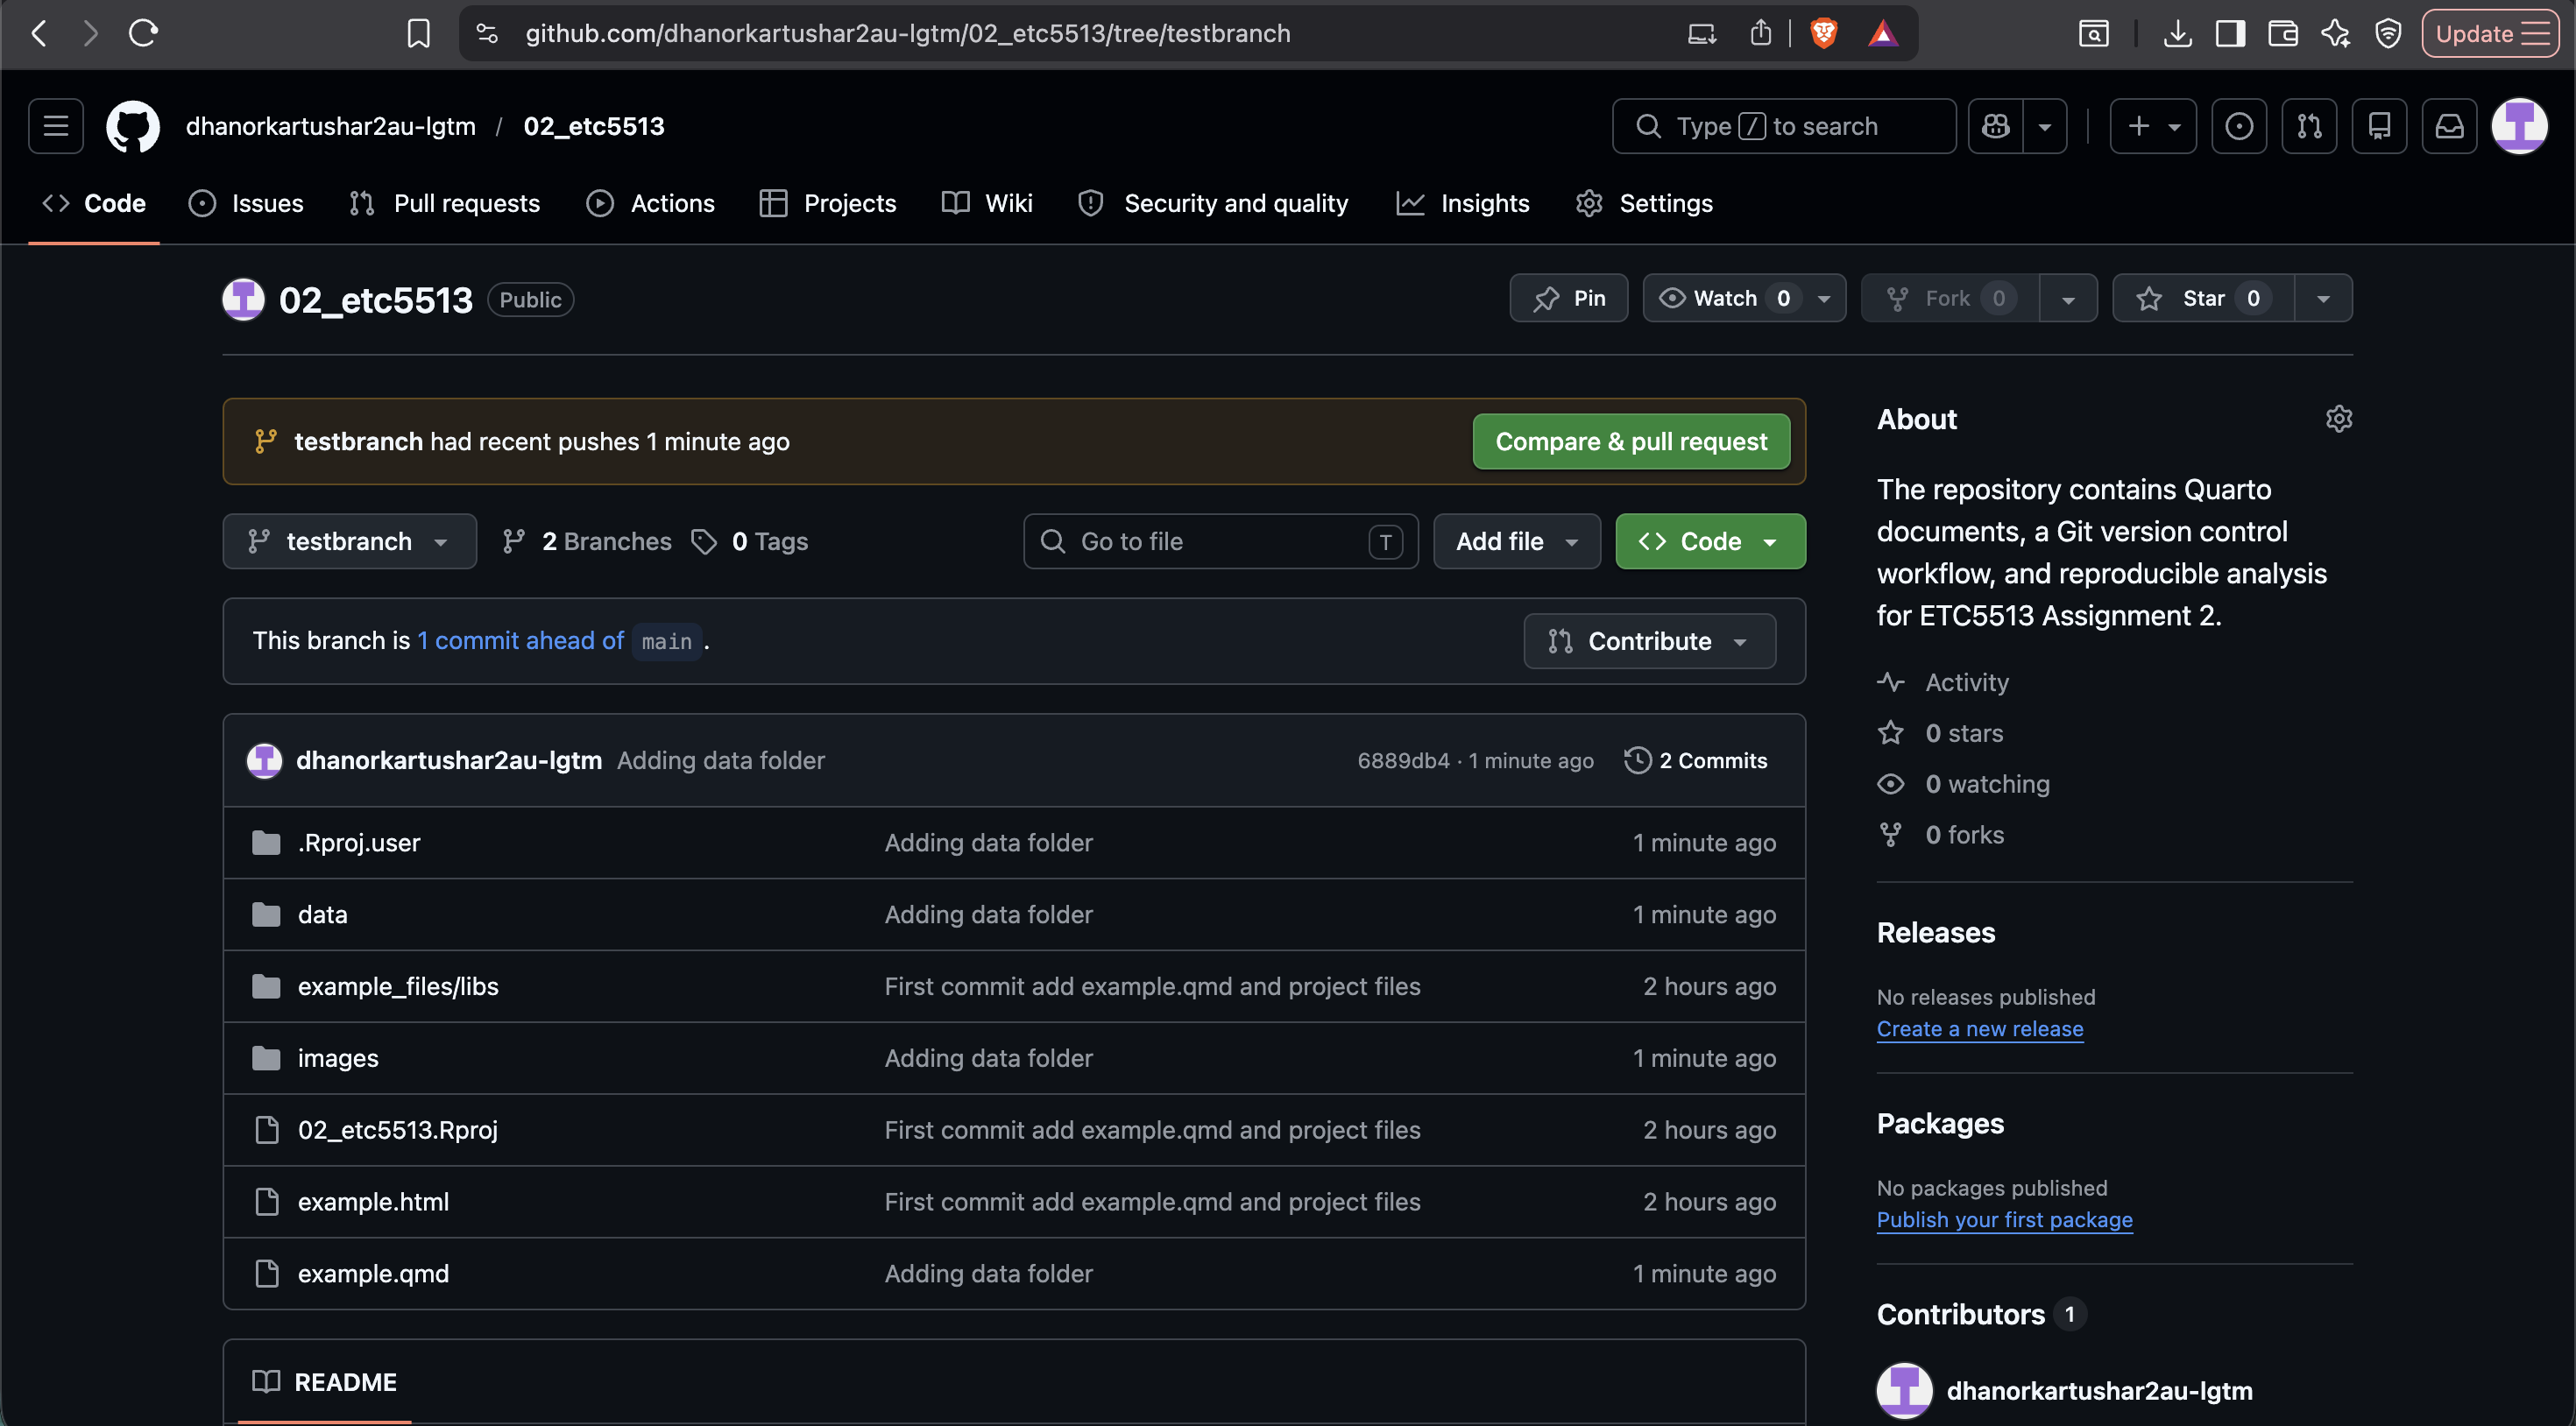
\includegraphics[keepaspectratio]{images/clipboard-163121543.png}}

\paragraph{\texorpdfstring{\textbf{Step 5:} Switch to \texttt{main} and
Create a Conflicting
Change:}{Step 5: Switch to main and Create a Conflicting Change:}}\label{step-5-switch-to-main-and-create-a-conflicting-change}

A merge conflict happens when \textbf{two branches modify the same part
of the same file in different ways}. Git doesn't know which version to
keep, so it asks you to decide manually.

In this step we \textbf{deliberately} creating that conflict by editing
the same part of \texttt{example.qmd} on \texttt{main} that we already
edited on \texttt{testbranch}

\begin{enumerate}
\def\labelenumi{\arabic{enumi}.}
\item
  \texttt{git\ checkout\ main} - Switched to branch `main'
\item
  \texttt{git\ branch} - Confirm we're on \texttt{main}
\end{enumerate}

Check what \texttt{example.qmd} looks like on \texttt{main}

Notice that when you switched to \texttt{main}, the changes you made on
\texttt{testbranch} are \textbf{gone from your files}. That's normal ---
each branch has its own version of the files.

Open \texttt{example.qmd} in RStudio. It should look like your original
version from Step 1, without the new section you added on
\texttt{testbranch}

\begin{enumerate}
\def\labelenumi{\arabic{enumi}.}
\item
  Modify \texttt{example.qmd} again

  \begin{itemize}
  \item
    Open \texttt{example.qmd} in RStudio and make a change to it. We are
    just changing the variable name i.e ``y''

\begin{Shaded}
\begin{Highlighting}[]
\NormalTok{y }\OtherTok{\textless{}{-}} \FunctionTok{c}\NormalTok{(}\DecValTok{10}\NormalTok{, }\DecValTok{20}\NormalTok{, }\DecValTok{30}\NormalTok{, }\DecValTok{40}\NormalTok{, }\DecValTok{50}\NormalTok{)}
\FunctionTok{mean}\NormalTok{(y)}
\end{Highlighting}
\end{Shaded}

\begin{verbatim}
[1] 30
\end{verbatim}
  \end{itemize}
\item
  \textbf{both branches are changing the same part of the file} but in
  different ways. Save the file.
\item
  Stage and commit the changes

  \begin{itemize}
  \item
    \texttt{git\ add\ example.qmd}
  \item
    \texttt{git\ commit\ -m\ "Add\ conflicting\ section\ to\ example.qmd\ on\ main"}
  \item
    \texttt{git\ push\ origin\ main}
  \end{itemize}
\item
  I switched back to the \texttt{main} branch using
  \texttt{git\ checkout\ main}. I then modified \texttt{example.qmd} by
  editing the same section that was changed on \texttt{testbranch}, but
  with different content --- deliberately creating a conflict for the
  next step. I staged the changes with \texttt{git\ add\ example.qmd},
  committed with a descriptive message, and pushed to GitHub using
  \texttt{git\ push\ origin\ main}
\end{enumerate}




\end{document}
